\documentclass[border=3pt]{standalone}
% Preâmbulo compartilhado pelos diagramas TikZ da aula 4 de Navegação (Representação de Mapas)
\usepackage[T1]{fontenc}
\usepackage[utf8]{inputenc}
\usepackage{lmodern}
\usepackage{amsmath}
\usepackage{xcolor}
\usepackage{tikz}
\usetikzlibrary{arrows.meta,angles,quotes,decorations.pathmorphing,decorations.pathreplacing,calc,
                positioning,shapes.geometric,shapes.misc,backgrounds,fit,
                math}

% Paleta (mesma dos SVGs originais)
\definecolor{dblue}{HTML}{2A5B8C}
\definecolor{dorange}{HTML}{B3541E}
\definecolor{dgreen}{HTML}{4A7C59}
\definecolor{dred}{HTML}{9C4B4B}
\definecolor{dcream}{HTML}{F4F1EA}
\definecolor{dshade}{HTML}{DDD7C9}

% Função gaussiana (não normalizada por padrão de escala visual)
\pgfmathdeclarefunction{gauss}{3}{%
  \pgfmathparse{1/(#3*sqrt(2*pi))*exp(-((#1-#2)^2)/(2*#3^2))}%
}

% Estilos comuns (prefixo d... para não colidir com chaves internas do pgf)
\tikzset{
  >={Stealth[length=2mm]},
  dguide/.style={gray!55, dashed, line width=0.4pt},
  daxis/.style={gray!60, line width=0.7pt, ->},
  dbody/.style={fill=black!3, draw=black!80, line width=1pt},
  dacc/.style={draw=dblue, line width=1pt},
  dlbl/.style={black!55, font=\small},
  dsub/.style={black!45, font=\footnotesize},
  dstate/.style={circle, draw=black!80, fill=dcream, line width=1pt,
                 minimum size=17mm, font=\large, inner sep=1pt},
  dobs/.style={circle, draw=black!80, fill=dshade, line width=1pt,
               minimum size=14mm, font=\large, inner sep=1pt},
  dbox/.style={rounded corners=2pt, draw=black!80, fill=dcream, line width=1pt,
               align=center, inner sep=6pt},
  dop/.style={circle, draw=black!80, fill=white, line width=1pt,
              minimum size=6mm, inner sep=0pt, font=\small},
  dtrans/.style={->, dblue, line width=1pt},
  dmeas/.style={->, dorange, line width=1pt},
  dcurve/.style={line width=1pt, dblue},
  dcurveb/.style={line width=1.4pt, dorange},
}

\begin{document}
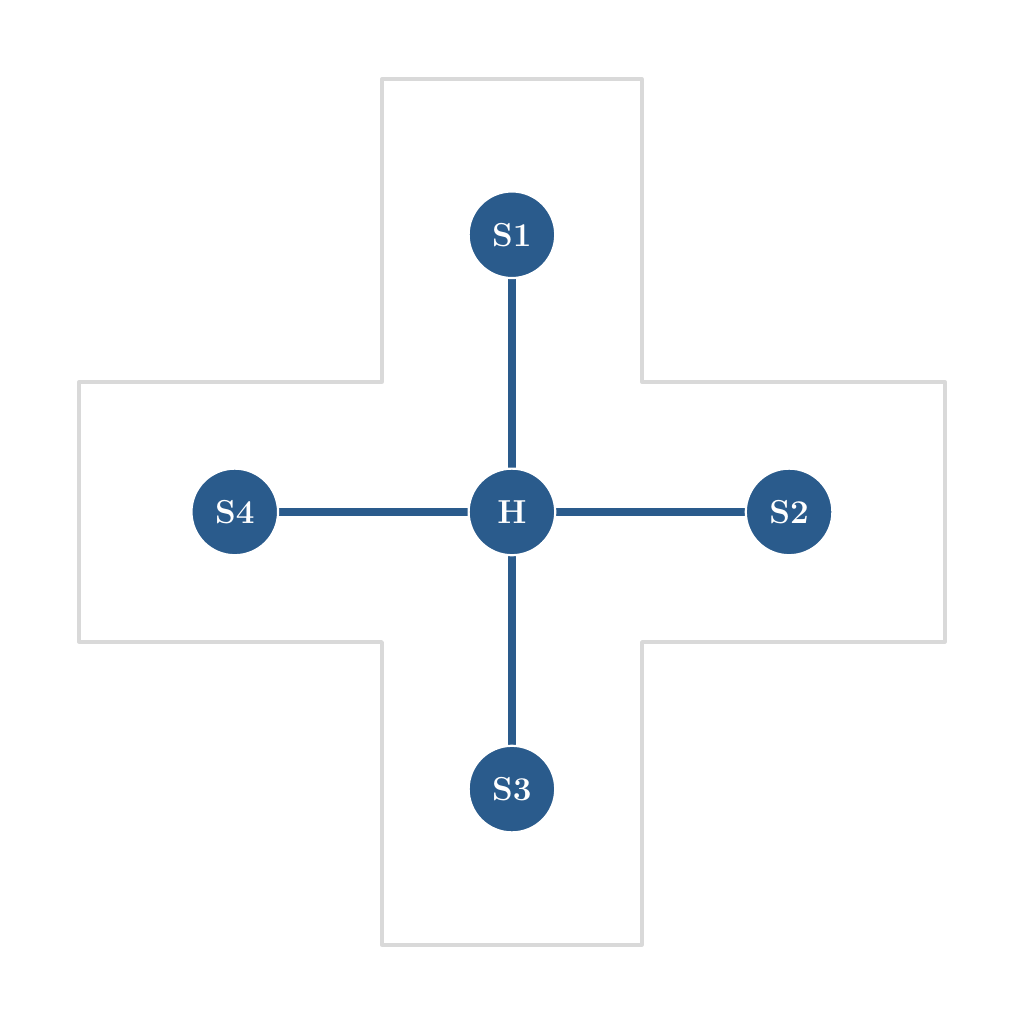
\begin{tikzpicture}[x=1cm,y=1cm]
\useasboundingbox (-0.1,-0.1) rectangle (12.2,12.2);
\draw[black!15, line width=1.2pt, line join=round] (4.40,0.55) -- (7.70,0.55) -- (7.70,4.40) -- (11.55,4.40) -- (11.55,7.70) -- (7.70,7.70) -- (7.70,11.55) -- (4.40,11.55) -- (4.40,7.70) -- (0.55,7.70) -- (0.55,4.40) -- (4.40,4.40) -- cycle;
\draw[dblue, line width=3pt] (6.05,6.05) -- (6.05,9.57);
\draw[dblue, line width=3pt] (6.05,6.05) -- (9.57,6.05);
\draw[dblue, line width=3pt] (6.05,6.05) -- (6.05,2.53);
\draw[dblue, line width=3pt] (6.05,6.05) -- (2.53,6.05);
\fill[dblue] (6.05,6.05) circle (0.55); \draw[white, line width=0.8pt] (6.05,6.05) circle (0.55); \node[white, font=\large\bfseries] at (6.05,6.05) {H};
\fill[dblue] (6.05,9.57) circle (0.55); \draw[white, line width=0.8pt] (6.05,9.57) circle (0.55); \node[white, font=\large\bfseries] at (6.05,9.57) {S1};
\fill[dblue] (9.57,6.05) circle (0.55); \draw[white, line width=0.8pt] (9.57,6.05) circle (0.55); \node[white, font=\large\bfseries] at (9.57,6.05) {S2};
\fill[dblue] (6.05,2.53) circle (0.55); \draw[white, line width=0.8pt] (6.05,2.53) circle (0.55); \node[white, font=\large\bfseries] at (6.05,2.53) {S3};
\fill[dblue] (2.53,6.05) circle (0.55); \draw[white, line width=0.8pt] (2.53,6.05) circle (0.55); \node[white, font=\large\bfseries] at (2.53,6.05) {S4};
\end{tikzpicture}
\end{document}
